\documentclass[12pt, onecolumn, letterpaper, oneside]{book}

\usepackage{authblk}
\usepackage[autostyle]{csquotes}
\usepackage{amsmath}
\usepackage{graphicx}
\usepackage{hyperref}
\usepackage[sc]{titlesec}
\usepackage{titlepic}

\usepackage[utf8]{inputenc}
\usepackage[T1]{fontenc}

\usepackage[square,numbers,sectionbib]{natbib}
\usepackage[sectionbib]{chapterbib}
\usepackage{titlesec}
\usepackage{indentfirst}

\usepackage{tikz}
\usepackage{rotating}

\usepackage{wasysym}

\titleformat{\chapter}[display]
  {\rmfamily\scshape\bfseries}{}{0pt}{\Large}
\titleformat{\section}[display]
  {\scshape}{}{0pt}{\large}
  
 \usepackage{scrextend}
 \interfootnotelinepenalty=10000

\usepackage{fancyvrb}
\usepackage{suffix}

\newcommand\chapterauthor[1]{\authortoc{#1}\printchapterauthor{#1}}
\WithSuffix\newcommand\chapterauthor*[1]{\printchapterauthor{#1}}

\usepackage{fancyhdr}
 
\pagestyle{fancy}
\renewcommand{\chaptermark}[1]{\markboth{}{\uppercase{\itshape #1}}}
\fancyhf{}
\fancyhead[L]{\rightmark}
\fancyhead[R]{\thepage}
\renewcommand{\headrulewidth}{0pt}
 
 \renewcommand\thefigure{\arabic{figure}}

\makeatletter
\newcommand{\printchapterauthor}[1]{%
  {\parindent0pt\vspace*{-25pt}%
  \linespread{1.1}\large\scshape#1%
  \par\nobreak\vspace*{35pt}}
  \@afterheading%
}
\newcommand{\authortoc}[1]{%
  \addtocontents{toc}{\vskip-10pt}%
  \addtocontents{toc}{%
    \protect\contentsline{chapter}%
    {\hskip1.3em\mdseries\scshape\protect\scriptsize#1}{}{}}
  \addtocontents{toc}{\vskip5pt}%
}
\makeatother

\title{Anarchao Discordia\\
		\vspace{1\baselineskip}
		\large{Vol. I}
		}
\date{Juillet, 2018\\
		 Confusion, YOLD 3184}
\author{Editeur: Griffensteed the 5$^\text{lth}$\\
			'Patafizikhood of Eris Esoteric\\}
\titlepic{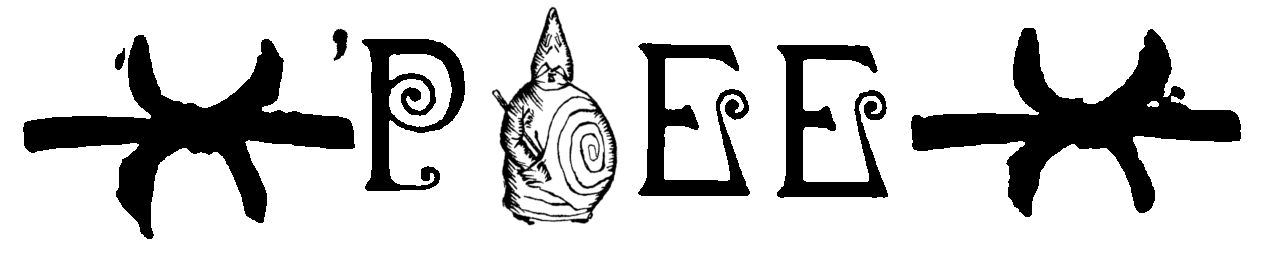
\includegraphics[scale=0.3]{./img/poee.png}}


\fancyfoot[L]{Confusion, YOLD 3184}
\fancyfoot[R]{Anarchao Discordia}

%\setlength\parindent{0pt}
    \setlength{\columnsep}{1cm}

\begin{document}
\sloppy
 \renewcommand{\contentsname}{Sommaire}

\maketitle

\tableofcontents

\chapter*{Notes}
\begin{verbatim}
La (re)découverte de l'anarchie par Discordia.
La (re)découverte de Discordia par l'anarchie.        
\end{verbatim}

\begin{center}
\emph{Dysnomie (Anarchie), Fille d'Eris.}\\
\end{center}

Le Discordianisme et l'Anarchie m'ont toujours semblé intrinsèquement liés par leurs origines, leurs idéologies, leurs auteurs, leurs vecteurs et leurs méthodes. Après avoir cherché à gauche à droite, il me parut que depuis 1990, avec la fin de \emph{No Governor}, édité par Robert Shea, aucune autre publication n'a réuni cette mère et cette fille, et j'ai senti le besoin de raviver cette flamme.\\
J'ai ressenti le besoin de (re)découvrir les anciens et les nouveaux penseurs anarchistes et discordiens et de regrouper leurs pensées et opinions ; de voir comment les anciennes idées des différentes parties de notre monde tiennent toujours fermement dans notre société actuelle ; d'exprimer de nouvelles idées sur les nouvelles opportunités et les nouveaux dangers qui surgissent et auxquels les anarchistes et les discordiens doivent se préparer.\\

\begin{center}
Anarchao Discordia\\
\end{center}

Ce premier volume d'\emph{Anarchao Discordia} se concentre principalement sur l'établissement des bases de ce à quoi les lecteurs pourront s'attendre à l'avenir. Il vise également à ``amorcer la pompe'' avec quelques grands articles d'auteurs célèbres, posant les fondations de l'anarcho-discordianisme, comme Robert Anton Wilson \& Robert Shea (p.4) et Gregory Hill (p.23) ; une excellente interview de Cornelius Castoriadis (traduit du français) sur la liberté et l'insignifiance de la politique moderne (p.25), considérée par Castoriadis comme une ``bouteille à la mer'' pour les générations futures (nous) ; un manifeste proto-discordien sur la musique de John Cage (p.32) ; et un article, par moi-même, sur une ``théorie mathématique du complot'' appliquée à la séparation des pouvoirs dans les démocraties représentatives (p.13).\\

Si vous vous sentez intéressé par ce projet, comme pour \emph{No Governor}, Anarchao Discordia a besoin de trois formes d'aide :
\begin{enumerate}
\item Il a besoin d'être lu. Les mots, les pensées et les idées ne peuvent vivre que s'ils atteignent les esprits. Je publie \emph{Anarchao Discordia} sous une licence GNU GPLv3, donc, s'il vous plaît, sentez-vous libre de le partager et distribuer comme vous le souhaitez.
\item Il a besoin d'articles. Si vous souhaitez exprimer votre opinion et vos idées sur la société, votre expérience, vos stratégies et solutions pour résoudre les fléaux des temps modernes, vos points de vue sur l'actualité, etc. avec un point de vue anarchiste et/ou discordien, veuillez nous contacter.
\item Il a besoin de commentaires et de critiques. Encore une fois, si vous voulez exprimer votre opinion sur cette revue, ce numéro ou les articles, n'hésitez pas à nous contacter.
\end{enumerate}

Mon but, si faisable, consisterait à publier un numéro de \emph{Anarchao Discordia} pour chaque saison discordienne. On verra comment ça se passe, mais en apprenant de \emph{No Governor}, ça peut apparaître difficile. Évidemment, j'ai mes propres biais en tant qu'anarcho-discordien, je me sens personnellement fortement attiré par les idées anarchistes de gauche et je ferai de mon mieux pour être conscient de ma propre grille de perception lorsque je ferai des jugements éditoriaux.

Vous pouvez nous contacter par email à : anarchao--at--discordia--dot--fr.

\par\begin{flushright} --- Griffensteed the 5$^\text{lth}$\\ Episkopos of the 'Patafizikhood of Eris Esoteric\end{flushright}

\chapter{Anarchisme et criminalité}
\chapterauthor{Robert Anton Wilson \& Robert Shea}

\emph{Cet article a été publié pour la première fois dans Green Egg, Vol. VII, No. 62, 1974.\\}

Comme les anarchistes visent l'abolition du gouvernement, la première question qu'on leur pose habituellement est la suivante : ``Qu'en est-il des meurtriers, des voleurs, des violeurs ? Le gouvernement nous protège d'eux. Les laisserais-tu faire librement ?\\
La réponse, tout d'abord, c'est que le gouvernement ne nous protège pas. Il s'agit d'une imposture totale, comme la fraude d'un chaman primitif qui prétend faire pleuvoir et avertit tout le monde : ``Si vous m'abolissez, il ne pleuvra plus jamais.'' Ainsi, \emph{les crimes majeurs sont tous légaux} ; les voleurs qui ont volé la terre et les ressources naturelles sous nos pieds opèrent avec une permission du gouvernement. Ces énormes banques, sociétés et monopoles fonciers financent les deux partis politiques, forment les avocats d'entreprises qui deviennent membres du Congrès ou présidents, et qui ne peuvent jamais être combattus avec succès devant les tribunaux parce qu'ils possèdent également les juges.\\
Deuxièmement, le prochain niveau de criminalité, le soi-disant Syndicate ou Mafia, est également de mèche avec les grands gouvernements et les grandes entreprises, et seules des arrestations symboliques et des peines légères ne sont imposées à leurs ``chefs des gangs'' --- généralement des rebelles devenus impopulaires auprès des mafieux de haut niveau. Dans toutes les grandes villes, les liens entre le bureau du maire et la mafia sont bien connus et souvent ``exposés'' dans la presse, mais aucune réforme n'est permanente et ne pourra jamais l'être dans le cadre de ce système. Les liens entre la mafia nationale et le gouvernement national sont moins bien médiatisés, mais certains livres comme \emph{La Politique de l'Héroïne en Asie du Sud-Est}, le récent volume de la revue Harpers sur la CIA et l'héroïne, etc. montrent que le réseau de l'héroine ne pourrait pas fonctionner sans une protection fédérale de haut niveau.\\
Finalement, le petit délinquant free-lance --- le violeur et voleur sournois --- peut être arrêté et poursuivi dans ce système ; mais, est-ce généralement le cas ? À New York, en 1972, il y a eu 300 000 cambriolages, mais seulement 20 000 arrestations pour cambriolage. La police est trop occupée à protéger les criminels de haut niveau --- comme nous l'expliquerons --- pour avoir le personnel nécessaire pour combattre les petits indépendants.\\
Vous niez cela ? Bien sûr, vous avez été formé par les écoles publiques et les médias pour le nier, croyez-vous en votre propre déni ? Dans quelle mesure vous sentez-vous en sécurité dans une grande ville américaine, surtout après la tombée de la nuit ? Pensez-vous honnêtement que le gouvernement peut vous protéger et qu'il le fera ?

\section*{Est-ce que plus de lois est la solution?}

Beaucoup admettent qu'ils sont effrayés et consternés par la vie moderne américaine, mais ils pensent que la réponse est plus de lois, des lois plus sévères, une évolution vers un État policier total.\\
Il s'agit, bien sûr, de l'orientation naturelle du gouvernement. Plus un politicien est honnête (et malavisé), plus il écrira des lois --- pour prouver à lui-même qu'il ``travaille'' pour le peuple. Évidemment, chaque fois que l'assemblée législative se réunit, les politiciens honnêtes présenteront plus de lois, pour montrer à quel point ils travaillent dur. Éventuellement, il ne restera plus rien qui ne soit couvert par une loi ou une autre. Tout ce qui n'est pas obligatoire sera interdit, et tout ce qui n'est pas interdit sera obligatoire.\\
Arrêtez-vous et demandez-vous si vous souhaitez vraiment ce genre de tyrannie, saveur Nazie ou Communiste.\\
Même si nous (ou la plupart d'entre nous) le voulons --- être protégés des criminels --- et même si nous accélérons nos progrès et adoptons un milliard de nouvelles lois par an, arrivant à la Loi Absolue dans cinq ou dix ans, que se passera-t-il alors ? Comment un tel système pourra-t-il être appliqué ? Kinsey a estimé que pour faire respecter nos lois sur les relations sexuelles, 95 \% de la population devrait devenir soit des policiers, soit des gardiens de prison, sauf qu'ils seraient tous, eux-mêmes, en prison. C'est déjà impossible, mais supposons que nous essayions aussi d'appliquer les lois sur la drogue et sur les jeux d'argent ? Nous passerions tous nos vies dans des prisons fédérales, passant une partie de la journée à garder les autres et une partie de la journée à être gardés par eux.\\
C'est absurde, mais dans le cadre d'un gouvernement et de la loi, comment pouvons-nous nous arrêter avant une société carcérale aussi totale ?\\
Et n'oubliez pas : chaque pas dans cette direction --- chaque nouvelle loi, et chaque nouvelle administration pour faire appliquer les nouvelles lois --- augmente votre fardeau fiscal. Déjà aujourd'hui, vous travaillez du 1er janvier au 23 mai pour le gouvernement fédéral, pour payer vos impôts pour l'IRS pour l'année. Pendant quelques mois, après ça, vous travaillez pour payer les impôts vexatoires, les imports d'État et les autres taxes cachées sur chaque produit que vous achetez, chaque film que vous regardez, chaque boisson que vous buvez. Il serait probablement moins cher de se laisser voler chaque semaine par un voleur de base. Le gouvernement est peut-être plus doux qu'un agresseur (parfois), mais il finit généralement par prendre plus d'argent.

\section*{Le rôle des lois}

Il y a trois sortes de lois dans les livres aujourd'hui, et les comprendre, c'est comprendre l'État. Le premier type de loi énonce le pouvoir de l'État sur vous. Elles disent : nous pouvons vous voler ceci par an (imposition), nous pouvons vous asservir pour cette période de temps (l'appel au jury), nous pouvons faire ceci et cela et vous ne pouvez pas résister parce que nous sommes vos Maîtres. Il s'agit des lois les plus ancienne : celles imposées à l'origine aux conquis par les conquérants. Aucune tentative de la justifier n'a jamais été convaincante pour quiconque a eu l'audace de les remettre en question. Elles sont basées sur la simple Force ; son seul argument est l'arme.\\
Le deuxième type de loi est la moralité coercitive. Cela fait de l'État un ecclésiastique armé. Elles énoncent que vous pouvez vous amuser de telle façon, mais pas de telle autre ; vous pouvez fumer ceci, mais pas cela ; vous pouvez boire ceci, mais pas cela. Tu ne joueras pas aux Petits Chevaux le soir de la pleine lune. Tu ne parieras pas le dimanche. Tu ne feras pas l'amour à ta femme de la façon qu'elle et toi le souhaitent, mais de la façon que les législateurs le décident. Quatre millions d'arrestations par an, et une incroyable dépense de temps, de main-d'œuvre et d'argent, sont consacrés à l'application de ces lois. Ce sont les lois qui établissent des crimes sans victimes. Ce sont les lois que tout le monde viole occasionnellement et certaines personnes violent constamment. Leur seule justification, comme pour le premier type de lois, est la force brute. C'est-à-dire, sans force, un homme qui croyait, disons, au régime végétarien adventiste du septième jour obéirait encore aux règles de ce régime ; avec force, les adventistes, s'ils entrent au gouvernement, peuvent tous nous y contraindre. Le jour n'est pas lointain où les fumeurs de marijuana prendront le dessus, et s'ils sont vengeurs, les lois contre l'alcool reviendront dans les lois. Cette stupide intimidation peut durer indéfiniment, chaque groupe ayant imposant à son tour ses propres préjugés aux autres. Les anarchistes disent : arrêtez maintenant, laissez votre voisin tranquille, lâchez-le et laissez tout le monde profiter de son propre style de vie.\\
Enfin, il y a la troisième type de lois --- le type dont toute personne décente souhaite que la société vive. Pas de meurtre. Pas de vol. Pas de viol. Pas de fraude. Les anarchistes, tout comme vous, aimeraient voir ces lois fonctionner réellement. Seulement, nous ne croyons pas que le gouvernement puisse faire ce travail. Nous pensons que le gouvernement est, a toujours été et sera toujours préoccupé par les deux premiers types de lois. Continuez à lire et nous vous expliquerons pourquoi.

\section*{La nature du gouvernement}

Le gouvernement a été institué pour garantir que les biens resteront volés. La fonction principale de chaque policier, chaque juge, chaque bureaucrate est de veiller à ce que les biens restent volés.
Les premiers rois étaient des conquérants. Ils ont volé la terre par balles et obus, un point c'est tout. Ensuite, ils se sont installés pour voler les survivants à un certain taux annuel, appelé imposition. Ensuite, ils ont divisé la terre avec leurs proches et leurs officiers de l'armée, qui sont alors devenus des seigneurs de la terre, des propriétaires terriens, et ont été habilités à voler les citoyens à un certain taux annuel, appelé loyer. Quand la science et l'industrie sont apparues, d'autres satrapes et flagorneurs des familles royales ont reçu des chartes pour monopoliser les ressources et les moyens de production, et pour voler à un certain taux par an, appelé le droit au capital ou profit. Quand les banques ont été créées pour faire circuler le moyen d'échange (l'argent), d'autres chartes ont été distribuées à d'autres membres du gang des bandits, qui sont devenus des directeurs de banque avec une licence pour voler à un autre taux par an, appelé intérêt monétaire ou intérêt économique.\\
Il est vite devenu évident que ceux qui ne faisaient pas partie du gang, c'est-à-dire la majorité de la population, étaient susceptibles de voler autant qu'ils le pouvaient. Le Robin des Bois apparaît dans toutes les sociétés à ce stade, et la plupart d'entre nous l'admirons encore, bien que honteusement, puisque les écoles et les médias nous disent de ne pas le faire. (Pourtant, qui n'héroïserait pas un peu Jesse James ou John Dillinger ?)\\
Les anarchistes disent que le premier crime a été le crime des conquérants/gouverneurs, qui se sont emparés des terres, l'ont répartie entre eux et nous ont tous volés à jamais par l'imposition, le loyer, le profit corporatif, l'intérêt monétaire et diverses sous-catégories de cette même fraude de base. Les anarchistes affirment que la Terre appartient à ses habitants, et non à cette petite classe ``propriétaire'' et ``gouvernante'' représentant moins de 1\%  de la population.\\
Les anarchistes affirment que la façon de stopper le crime est de stopper le crime primordial, l'État et d'administrer la terre par le biais d'associations volontaires (syndicats) par le peuple.\\
Les anarchistes affirment que si les gens pouvaient travailler pour eux-mêmes --- s'ils recevaient le plein produit de leur travail par l'intermédiaire d'un syndicat de camarades travailleurs --- presque toute motivation pour le crime disparaîtrait. Si vous n'aviez pas à payer les impôts et le loyer, à partir de demain, votre pouvoir d'achat serait plus que doublé. Si d'autres formes d'exploitation et de vol, par le biais du système de l'intérêt financier, étaient également abolies, votre pouvoir d'achat serait plus que quadruplé. Combien d'envie, combien d'inquiétude au sujet de l'argent, combien de peur irrationnelle, d'ulcères, de cauchemars, de maux de tête et d'autres motivations pour tricher un peu ou voler un peu survivraient après cette simple justice économique ?

\section*{Les autres criminels}

``Mais, mais --- qu'en est-il des criminels violents ? Qu'en est-il des tueurs passionnels, des fous, des psychopathes ou des sociopathes ou des sadiques ? Ou ceux qui aiment simplement être maléfique et destructeur ?''\\
Nous n'éludons pas cette question. Il est absolument nécessaire, cependant, de le mettre en perspective en expliquant le Crime Économique Majeur du gouvernement capitaliste (et des gouvernements féodaux et autres) et comment d'autres crimes moins graves découlent surtout de cette injustice primordiale.\\
Même après que la justice économique soit réalisée et que des associations bénévoles de toutes sortes (syndicats, coopératives de crédit, coopératives de consommateurs, compagnies d'assurance appartenant à des personnes, communes rurales, tribus, tout type de groupement humain libre) aient repris les fonctions du gouvernement, \emph{quelques} personnes, pour cause de maladie ou de perversité ou quelques autres fichues raisons, continueront de créer des emmerdes. Viol. Vol. Tentatives de fraude. Comment les anarchistes vont-ils s'y prendre avec les malfaiteurs restants?

\section*{L'éducation et la famille}

La première étape dans la résolution de tout problème social, comme tout problème médical, est la prévention. Les autres remèdes ne sont nécessaires qu'en cas d'échec de la prévention.\\
Les anarchistes prétendent que l'être humain fou-furieux est produit par nos méthodes actuelles d'éducation des enfants. Cette affirmation n'est guère radicale ou extrême : chaque psychiatre, chaque sociologue, chaque anthropologue, d'une manière ou d'une autre, admet que cette accusation grave est vraie. Nous n'aurions pas autant de violeurs et d'autres nuisances violentes si notre société n'était pas, d'une certaine façon, en train de les entraîner dès la naissance à se comporter ainsi. Par exemple, la Suède n'a que quelques viols par an ; les États-Unis en ont un toutes les sept minutes. Un viol toutes les sept minutes n'est pas un comportement masculin naturel (quoi qu'en dise les mouvements féministes) ; c'est une conséquence de la misère sexuelle dans cette société.\\
Les anarchistes pensent que les pratiques répressives, autoritaires, coercitives, brutales et dégradantes actuellement utilisées dans la famille et à l'école ne sont nécessaires que pour conditionner le jeune humain à vivre dans une société dirigée par un gouvernement. Les enfants doivent être battus ou terrorisés et intimidés à la maison et à l'école afin qu'ils puissent s'adapter à la terreur et à la brutalité du gouvernement à mesure qu'ils grandissent. En bref, une société d'État doit être répressive parce que la répression est l'essence même de l'État.\\
Les familles et les écoles libertaires et libres --- la famille ouverte, l'école de Summerhill, la libre association d'hommes, de femmes et d'enfants sans contrôle autoritaire --- ne produiront pas les types déformés, tordus mentalement, violents et ``méchants'' et ``fous'' si courants dans notre société autoritaire. Les anarchistes visent donc, tout d'abord, à empêcher les criminels violents en changeant les méthodes d'éducation des enfants qui les engendrent.

\section*{Le démoniaque ou le monstre}

Il reste encore l'inexplicable criminel --- le gars qui aime faire du mal aux autres pour des raisons que personne aujourd'hui ne peut comprendre. Les superstitieux disent qu'il est possédé par des démons ; les naturalistes laissent entendre qu'il a peut-être de mauvais gènes ou qu'il est de retour à un stade antérieur de l'évolution. Quelle qu'en soit l'explication, ce gars apparaîtra, probablement dans les sociétés anarchistes, comme il est apparu dans toutes les autres sociétés, même après l'abolition de l'injustice économique et de l'éducation de l'esprit.\\
Les sociétés centrées sur l'Homme (par opposition aux sociétés gouvernementales ou centrées sur la propriété) s'occupent de ce problème depuis des milliers d'années. Tribus, clans, bandes, communes libres, ont existé en marge, avant et aux côtés des États qui reçoivent toute l'attention des historiens. Les anthropologues ont enquêté sur ces groupes d'humains libres et ont trouvé une variété de méthodes pour faire face aux ``démoniaques'', dont beaucoup sont aussi bonnes voire meilleures que les prisons traditionnelles étatiques, les tortures ou les exécutions.\\
L'ostracisme ne doit pas être sous-estimé. Un critique de l'anarchisme, George Orwell, s'est en fait plaint que l'ostracisme était si cruel que la plupart des gens préféreraient tomber en prison plutôt que d'être la seule personne ostracisée dans une communauté anarchiste.\\
L'exil, largement utilisé par les gouvernements avant que la prison ne devienne populaire, est également efficace. Au moins, il résout le problème pour la communauté qui l'utilise (tout en transmettant, hélas, le problème à la communauté malchanceuse qui aura à son tour le fou-furieux).\\
Les Quakers ont largement pratiqué une forme de pardon moral qui semble peu pratique pour la plupart d'entre nous, mais qui est d'une efficacité meurtrière. Bertrand Russell a été tellement impressionné par cela qu'il l'a suggéré comme une punition convenable pour Staline. Tant que vous n'avez pas vu un groupe de Quakers réciter les péchés de quelqu'un en public, pleurer à haute voix, puis pardonner et prier pour le coupable, vous ne pouvez pas imaginer l'impulsion psychologique que cela génère.\\
Beaucoup d'anarchistes croient que les groupes de défense privés sont légitimes ; certains sont même prêts à permettre à de tels groupes d'utiliser les méthodes traditionnelles des Vigilante. Clarence Lee Schwartz, un anarchiste américain qui a observé ce système de première main dans l'ancien Occident, pensait qu'il était à la fois plus humain et plus efficace pour le maintien de la paix que le système de droit du gouvernement dans l'Est. D'autres anarchistes craignent cependant que ce soit la source possible d'un nouvel État.\\
La plupart des anarchistes croient que les criminels ne devraient en aucun cas être mis en cage, en raison des preuves accablantes que chaque prisonnier sort d'une cage pire que lorsqu'il y entre. D'autres croient, cependant, que la punition sous forme d'indemnisation est compatible avec les idées libertaires et devrait être rigoureusement appliquée par des syndicats anarchistes. En vertu du système d'indemnisation, tout criminel doit payer en espèces ou en travail ou en biens nécessaires pour indemniser ses victimes (ou leurs survivants). Cela fait certainement plus de bien aux victimes que de voir le criminel mis en cage et nourri aux frais de la communauté, c'est le moins que l'on puisse dire ; et c'est probablement tout autant décourageant ou encore plus décourageant pour les fous à qui il reste une capacité de prévoir les conséquences probables de ses actions.\\
Enfin, il faut mentionner quelques solutions diverses. Tout comme le crime dans une communauté économiquement juste et libre sera anormal et sporadique (plutôt que la terreur constante d'heure en heure que c'est dans cette société folle, inégale et non libre), les remèdes seront également individualisés et propres à chaque situation. Dans certains cas, sans aucun doute, une communauté anarchiste décidera que le ``criminel'' avait raison et que la communauté avait tort ; pour cette raison, les anarchistes ne croient pas aux lois inaltérables, mais seulement aux principes généraux.\\
L'apogée de la théorie anarchiste est le principe de non-invasivité ou de non-coercition --- Occupez-Vous de Vos Affaires --- et ceux qui enfreignent cette règle devront, en général, indemniser ceux dont la vie a été endommagée. S'ils refusent, des méthodes comme le boycott, l'ostracisme, l'exil, ou le mauvais accueil généralisé peuvent être ou ne pas être délibérément organisées contre eux. Le bon sens, les liens sociaux et le sens de l'humour de la communauté organique trouveront un moyen de leur faire savoir que la tolérance humaine, même sous l'anarchie, n'est pas infinie. Dans le vieil Ouest, les hommes qui avaient parcouru la ville avec un putois attachée autour du cou, puis qui avait été poussé sur l'autoroute, sont souvent devenus des citoyens précieux, coopératifs et productifs dans la ville voisine, après un certain temps pour évaluer la probabilité d'une répétition de cet amusement public s'ils essayaient de nouveau des modes de comportement similaires.

\chapter[Coalitions et séparation des pouvoirs]{RAW, Eric Temple Bell, la Loi des Cinq, coalitions et séparation des pouvoirs}
\chapterauthor{Griffensteed the 5$^\text{lth}$}

\blockquote{
\small{``Ce que Weishaupt découvrit cette nuit du 2 février, dix-sept soixante-seize," expliqua Hagbard Celine à Joe Malik en 1973, par une claire journée d'automne à Miami, à peu près au même moment où le capitaine Tequilla y Mota lisait Luttwak sur le coup d'État et faisait ses premiers pas vers la cabale de l'officier qui a ensuite saisi Fernando Poo,``était essentiellement une simple relation mathématique. C'est si simple, en fait, que la plupart des administrateurs et des bureaucrates ne le remarquent jamais. convoitise, tel le propriétaire ne remarque pas l'humble termite, jusqu'à ce qu'il soit trop tard. . . . Tiens, prends ce papier et fais-toi une idée. Combien de permutations y a-t-il dans un système à quatre éléments ?

Joe, se souvenant des mathématiques de lycée, écrivit $4\times3\times3\times2\times1\times1$, et lut à haute voix sa réponse ``vingt-quatre''.

``Et si tu es l'un des éléments, le nombre de coalitions --- ou pour être sinistre, de conspirations --- que tu pourrais avoir à affronter serait de vingt-trois. Malgré les obsessions de Simon Moon, le vingt-trois n'a pas de signification mystique particulière," ajouta rapidement Hagbard. ``Il s'agit d'un certain nombre de relations possibles dont le cerveau peut se souvenir et gérer. Mais supposons maintenant que le système comporte cinq éléments . . . ?.''

Joe écrivit 5$\times4\times3\times3\times2\times1$ et lut à haute voix, ``Cent vingt-et-un."

``Tu vois ? On rencontre toujours des sauts de cette taille lorsqu'il s'agit de permutations et de combinaisons. Mais, comme je l'ai dit, en règle générale, les administrateurs n'en sont pas conscients. Korzybski a fait remarquer, au début des années trente, que personne ne devrait jamais superviser directement plus de quatre subordonnés, parce que les vingt-quatre coalitions possibles que la politique de bureau ordinaire peut créer suffisent à taxer n'importe quel cerveau. Quand il saute à cent vingt, l'administrateur est perdu. C'est là, par essence, l'aspect sociologique de la mystérieuse Loi des Cinq. Les Illuminati ont toujours cinq dirigeants dans chaque nation, et cinq Illuminati Primi internationaux qui les supervisent tous, mais chacun dirige son propre spectacle plus ou moins indépendamment des quatre autres, unis seulement par leur engagement commun à l'Objectif du Gruad." Hagbard s'arrêta pour rallumer son long cigare italien noir.}
\par\begin{flushright} \textup{--- Robert Shea \& Robert Anton Wilson}, Illuminatus!, 1975. \end{flushright}
}

\begin{center}

\includegraphics[scale=0.1]{./img/eris.png}
\end{center}

\section*{Combinatoire des coalitions}
Contrairement à ce qu'explique Hagbard Celine dans cet extrait introductif, le nombre de coalitions --- ou, pour être sinistre, de conspirations --- que l'on peut obtenir avec un système de $n$ éléments n'est pas lié au nombre de permutations mais a plutôt rapport avec le problème de partition d'un ensemble ; un autre problème de combinatoire définit par une relation mathématique plus complexe.\\

D'une part, le nombre de permutations de $n$ éléments correspond au nombre de façons de disposer ces $n$ éléments dans une ligne \cite{Graham1988}. Par exemple, pour l'ensemble $\{1,2,3\}$ il y a six permutations possibles :
\begin{gather*}
(1,2,3) \qquad (1,3,2) \qquad (2,1,3) \\ 
(2,3,1) \qquad (3,1,2) \qquad (3,2,1)
\end{gather*}
Dans ce cas, Joe Malik a fait le calcul correct lorsqu'il s'agissait de permutations, en suivant les instructions de Hagbard. Il y a $n$ choix pour le premier élément, $n-1$ pour le deuxième, $n-2$ pour le troisième, et ainsi de suite, donnant $n\times(n-1)\times(n-2)\times(n-2)\times...\times1$, c'est à dire
\begin{equation}
n ! = \prod\limits_{k = 1}^n k
\end{equation}
La séquence entière des nombres factoriels (commençant par $0!$) est : $1, 1, 1, 2, 6, 24, 120, 720, ....$ (séquence A000142 sur l'Encyclopédie en ligne des séquences entières\footnote{\url{https://oeis.org}}).
Cependant, les permutations ne montrent que des façons d'organiser les éléments, mais ne traitent pas des différentes façon de regrouper les éléments et ne sont donc pas un bon modèle pour traiter des coalitions.\\

D'autre part, une partition d'un ensemble $S$ constitué de $n$ éléments est une famille de sous-ensembles de $S$ disjoints appelés ``blocs'' dont l'union est $S$ \cite{Rota1964}.
En d'autres termes, elle correspond à une façon de regrouper tous les éléments de l'ensemble en sous-ensembles, c'est-à-dire les différentes coalitions possibles avec $n$ éléments. Par exemple, pour l'ensemble $\{1,2,3\}$, il y a cinq partitions possibles :
\begin{gather*}
(\{1\},\{2\},\{3\}) \quad (\{1,2\},\{3\}) \quad (\{1,3\},\{2\}) \\
(\{1\},\{2,3\}) \quad  (\{1,2,3\})
\end{gather*}
Compter le nombre de partitions d'un ensemble avec $n$ éléments est un peu plus compliqué. Il correspond au nombre de Bell $B_n$, nommé d'après le mathématicien Eric Temple Bell, et peut être calculé à l'aide de la formule récursive suivante :

\begin{equation}
    \begin{cases}
         B_0 = 1\\
         B_{n+1} = \sum\limits_{k=0}^n \binom nk B_k \quad \text{.}
     \end{cases}
\end{equation}
La démonstration de cette formule et d'autres formules pour les nombres de Bell peut se trouver dans \cite{Graham1988, Rota1964}.
Une autre méthode pour calculer les nombres de Bell consiste à construire le triangle de Bell \cite{Aitken1933}. Ce triangle est construit en suivant les règles suivantes :
\begin{itemize}
\item commencer par le chiffre 1,
\item pour chaque nouvelle ligne, la valeur la plus à gauche est une copie de la valeur la plus à droite de la ligne précédente,
\item toutes les autres valeurs sont la somme de la valeur à sa gauche et de celle en diagonal en haut à gauche.
\end{itemize}
 Les premières rangées du triangle de Bell sont illustrées dans la Figure \ref{bell}. La séquence entière des nombres de Bell (à partir de $B_0$) est : $1, 1, 1, 2, 5, 15, 52, 203, ....$ (séquence A000110 sur l'OEIS).\\

\begin{figure}[h]
\begin{center}
 \[ 
    \begin{matrix}
    1 & & & & & & & \longrightarrow & B_1= 1\\
    1 & 2 & & & & & & \longrightarrow & B_2= 2\\
    2 & 3 & 5 & & & & & \longrightarrow & B_3= 5\\
    5 & 7 & 10 & 15 & & &&  \longrightarrow & B_4= 15\\
    15 & 20 & 27 & 37 & 52 & & & \longrightarrow & B_5= 52\\
    52 & 67 & 87 & 114 & 151 & 203 & & \longrightarrow & B_6= 203\\    
    \vdots\\
    \end{matrix}
\]
\caption{\label{bell} Premières lignes du triangle de Bell.}
\end{center}
\end{figure}

Les choses se compliquent encore plus si l'on considère que les partitions peuvent être ordonnées. Dans ce cas, les différentes permutations d'une partition donnée doivent être prises en compte. C'est ce qu'on appelle un ordonnancement faible et cela peut être utilisé pour déterminer le nombre de façons de classer $n$ joueurs lorsque les \emph{ex-aequo} sont possibles \cite{Good1975}. Dans notre cas, il peut être utilisé pour représenter les relations de pouvoir déséquilibrées entre les différents éléments/coalitions. Par exemple, pour l'ensemble $\{1,2,3\}$, il y a treize \emph{partitions ordonnées} possibles :
\begin{gather*}
(\{1\},\{2\},\{3\}) \quad (\{1\},\{3\},\{2\}) \\ 
(\{2\},\{1\},\{3\}) \quad (\{2\},\{3\},\{1\}) \\ 
(\{3\},\{1\},\{2\}) \quad (\{3\},\{2\},\{1\}) \\
(\{1\},\{2,3\}) \quad (\{2,3\},\{1\}) \quad (\{2\},\{1,3\}) \\
(\{1,3\},\{2\}) \quad (\{3\},\{1,2\}) \quad (\{1,2\},\{3\}) \\
(\{1,2,3\})
\end{gather*}
Le nombre de partitions ordonnées possibles d'un ensemble d'éléments $n$ est donné par les nombres de Bell ordonnés (aussi appelés nombres de Fubini), définis par \cite{Knuth1998} :
\begin{equation}
     a_n= \sum\limits_{k=0}^n k ! S(n,k) \quad \quad \text{,}
\end{equation}
où $S(n,k)$ est le nombre de Stirling de seconde espèce, correspondant au nombre de façons de partitionner un ensemble de $n$ éléments en $k$ sous-ensembles non vides, et peut être calculé avec la formule récursive \cite{Graham1988} :
\begin{equation}
    \begin{cases}
    S(0,0) = 1 \quad \text{and} \quad S(0,n) = S(n,0) = 0\\
    S(n+1,k) = kS(n,k) + S(n,k-1)
    \end{cases}
\end{equation}
La séquence entière des nombres de Bell ordonnés (à partir de $a_0$) est : $1, 1, 1, 3, 13, 75, 541, 4683, ....$ (séquence A000670 sur l'OEIS).

\section*{Les répercussions}

De retour à nos coalitions --- ou pour être sinistre, conspirations --- et à l'extrait d'\textit{Illuminatus!} Si nous considérons d'abord les partitions non ordonnées : ``Combien de partitions différentes y a-t-il dans un système à quatre éléments ?", aurait dû demander Hagbard Céline.\\
Joe écrivit le début de la séquence des nombres de Bell et lut à haute voix ``le quatrième nombre de Bell est quinze."\\
Donc, si on supprime l'état où tous les éléments sont séparés, c'est-à-dire sans coalition, cela signifie que le nombre de coalitions possibles avec quatre éléments auxquels on pourrait avoir à faire serait de quatorze\footnote{$1+4=5$, mais oublions la magick de la Loi des Cinq\cite{Malaclypse1963}.}. Et maintenant, qu'en est-il d'un système à cinq éléments ?\\
Joe lut à haute voix ``le cinquième nombre de Bell est cinquante-deux."\\
De même, le nombre de coalitions possibles avec cinq éléments auxquels on pourrait avoir à faire serait de cinquante et un. La Figure \ref{part} montre les 52 différentes partitions possibles pour un ensemble de 5 éléments.
Dans ce cas, même si le problème n'a pas été correctement résolu par l'utilisation de permutations au lieu de partitions, la déduction de RAW et de Korzybski est toujours valable. 
Le saut de quatorze à cinquante et une relations possibles est suffisant pour passer de quelque chose d'épuisant pour l'esprit à quelque chose d'assez grand pour le perdre complètement \cite{Kelly1955, Korzybski1933}. \\

\begin{figure}
\begin{center}
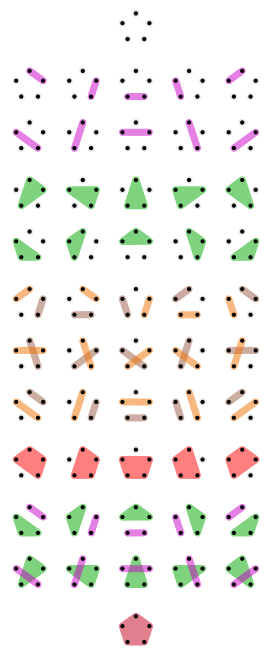
\includegraphics[scale=0.7]{./img/part.png}
\caption{\label{part} Les 52 partitions d'un ensemble à 5 elements (source: wikipedia).}
\end{center}
\end{figure}

Maintenant, si nous considérons les partitions ordonnées, le saut apparaît plus tôt. Le troisième nombre de Fubini est treize et le quatrième nombre de Fubini est soixante-quinze \footnote{$75=5\times 15$ }. De plus, dans ce cas, toutes les configurations sont problématiques, puisqu'elles représentent soit des coalitions, soit des rapports de force déséquilibrés entre les éléments. Avec ce modèle, la déduction de RAW et de Korzybski apparaît plus tôt qu'ils ne l'ont formulé en termes de nombre d'éléments ; quatre éléments devenant le nouveau point de basculement.


\section*{La Loi des Cinq et la séparation des pouvoirs}

Lorsqu'ils expriment les bases nécessaires pour obtenir une véritable démocratie, John Locke et Montesquieu identifient le besoin de séparation des pouvoirs (c'est-à-dire l'absence de coalition entre les pouvoirs) pour les \textit{démocraties représentatives} dans leurs essais respectifs \textit{Traité du gouvernement civil} \cite{Locke1689} et \textit{De l'esprit des lois} \cite{Montesquieu1748}. De plus, les critiques modernes de leurs travaux, lorsqu'il s'agit de l'établissement d'une démocratie, visent d'abord le fait que les organisations proposées respectivement par Locke et Montesquieu n'assurent pas une réelle séparation des pouvoirs mais plutôt une interdépendance des pouvoirs ; puis le fait que les différents pouvoirs identifiés ne sont pas mis sur un pied d'égalité, certains étant plus importants que d'autres.\\

Montesquieu identifie trois pouvoirs \cite{Montesquieu1748}, qui sont maintenant représentés par différentes institutions dans de nombreuses démocraties représentatives à la suite du \textit{Siècle des Lumières} :
\begin{itemize}
\item le pouvoir législatif,
\item le pouvoir exécutif,
\item le pouvoir judiciaire.
\end{itemize}
Dans ce contexte avec trois pouvoirs, le troisième nombre de Bell nous indique que le nombre de coalitions possibles (et donc l'absence de réelle séparation des pouvoirs) est de quatre ($B_3 - 1$), et le troisième nombre de Fubini nous indique que le nombre de coalitions possibles ou de relations de pouvoir déséquilibrées (et donc l'absence de véritable séparation des pouvoirs ou d'égalité entre pouvoirs) est de treize ($a_3$).\\
En d'autres termes, avec les deux modèles, nous obtenons un certain nombre de relations possibles que le cerveau, les institutions et les gens peuvent gérer.
Il serait donc théoriquement possible d'obtenir une véritable démocratie avec une démocratie représentative.\\

Cependant, de nouveaux pouvoirs ont été identifiés depuis. En particulier :
\begin{itemize}
\item le pouvoir médiatique (aussi appelé ``le quatrième pouvoir'') \cite{Bourdieu1996, Herman1988},
\item le pouvoir économique (aussi appelé ``le cinquième pouvoir'') \cite{Ramonet1989, Ramonet1996}.
\end{itemize}
L'ajout de ces deux pouvoirs change radicalement la donne. Avoir cinq pouvoirs signifie que le nombre de coalitions possibles est donné par le cinquième nombre de Bell, c'est-à-dire cinquante-et-un ($B_5 -1$), et le nombre de coalitions possibles ou de relations de pouvoir déséquilibrées est de cinq cent quarante-et-un ($a_5$).\\
Cette situation devient alarmante parce qu'en plus de ne pas avoir d'institutions pour aider à la séparation de ces nouveaux pouvoirs avec les autres (puisque les institutions ont été créées avant leur identification), le nombre de coalitions possibles et de relations de pouvoir déséquilibrées devient beaucoup trop lourd à gérer pour le cerveau, les institutions et le peuple. De plus, cette question ne peut qu'empirer à mesure que de nouveaux pouvoirs sont identifiés (on pourrait, par exemple, ajouter Internet et l'opinion publique\footnote{$B_6 = 203$ et $a_6 = 4683$.}) avec des sauts devenant de plus en plus grands.\\

\section*{Conclusion}

Pour ces raisons, je conclurais que la séparation des pouvoirs n'est pas une base suffisante pour obtenir une véritable démocratie. Par conséquent, les démocraties représentatives ne sont pas des systèmes politiques viables puisqu'elles ne peuvent pas empêcher un règne de pouvoir(s) et n'encouragent que la création de nouvelles aristocraties de têtes grises et le totalitarisme. 
J'encourage donc les membres de \textsc{The House of the Rising Collapse} à lancer un \textit{Mouvement Eristique pour Dysnomie, Fille de Déesse} dont l'objectif principal est la dissolution totale de toute forme de pouvoir et l'acquisition d'une démocratie directe.

\begin{center}
\textit{Ne les laissez pas immanentiser l'eschaton !\\}

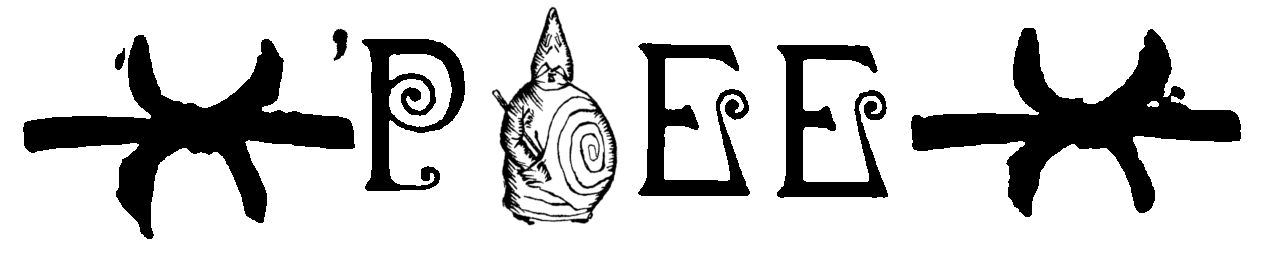
\includegraphics[scale=0.3]{./img/poee.png}
\end{center}

\section*{Remerciements}
Cet article a été écrit pour la \emph{Patafizikhood of Eris Esoteric}. Il n'a PAS été réalisé avec le support de l'AISB. Consultez votre glande pinéale. \textsc{Gloire à Discordia!!!!!}

%References
\bibliographystyle{unsrt}
\bibliography{coalitions_biblio}

\chapter{Pourquoi je ne suis pas un anarchiste}
\chapterauthor{Gregory Hill}

\emph{Cet article a été publié pour la première fois dans No Governor, Vol. I, No. 2, 1975.\\}

Il y a environ cinq ans, je me considérais comme un anarchiste (anarcho-pacifiste, en particulier), parce que je crois que la plus haute autorité disponible pour tout individu est sa propre expérience sincère et que toute autre autorité ne fournit au mieux que des informations indirectes.\\
Je n'ai pas changé d'avis à ce sujet, mais j'ai cessé de me qualifier comme anarchiste. La raison en est simple et basique : \textsc{trop de putain de règles}.\\
OK, c'est une blague. Mais c'est une blague \textsc{vraie}. L'incompatibilité n'est pas entre ma position et certaines théories anarchistes, mais entre ma position et la position de la plupart de ceux qui utilisent l'étiquette ``anarchiste."
Il semble que la Règle Numéro Un de l'anarchie, telle qu'elle est comprise par les autoritaires et par la plupart de ceux qui se disent anarchistes, est qu'un gouvernement est un ennemi. La Règle Numéro Deux est que pour obtenir la liberté, l'individu est politiquement ou moralement ou d'une manière ou d'une autre obligé de combattre cet ennemi.\\
À mon avis, ces règles représentent une position qu'il vaudrait mieux qualifier d'anti-archie. Le préfixe ``an" signifie "sans" et n'implique pas nécessairement ``contre". Il y a un parallèle exact avec le mot athéisme --- il est habituellement utilisé et compris, par ceux qui sont pour et contre, comme si le mot était anti-théisme.\\
Je peux respecter la position anti-archiste, mais je ne la partage pas. Le gouvernement n'est pas mon ennemi parce qu'il n'y a pas de gouvernement. OK, c'est une autre blague, mais c'est encore une blague \textsc{vraie}. Je sais bien qu'il y a des gens armés qui restreignent ma liberté de décision, et je connais des groupes de gens qui perçoivent des impôts auprès de moi, et tout le reste de ce gouvernement le perçoit de la même manière que je perçois (par exemple) un gros rocher sur mon chemin qui m'oblige à faire un pas de côté et à m'adapter. Franchement, je ne crois pas non plus aux rochers --- Je me contente de faire un pas et de m'adapter (ce qui est en fait plus facile que de croire en eux). Je pense qu'il y a une grande différence de niveau entre (a) répondre existentiellement à un phénomène et (b) le conceptualiser comme un ``ennemi". Si tout ce qui, dans l'univers, a déjoué mon dessein est mon ennemi, rien ne peut être mon ami --- et cela m'exclut moi-même. Mais, tout de même, je respecte la position anti-archiste. Après tout, si l'on perçoit un phénomène comme étant un ennemi, alors on serait un fou de faire autre chose que de se défendre.\\
Le gros de cet essai est de pinailler sur les étiquettes. Pourtant, je me sens libre de pinailler, et en tout cas ce que j'essaie de faire, c'est d'éviter que d'autres pensent que je suis en guerre avec certaines personnes simplement parce que ces personnes pensent qu'elles sont un gouvernement et font tout ce qu'elles peuvent pour m'imposer leurs notions par la force.\\
Je ne suis pas en guerre avec eux ni avec les rochers. Et dans la mesure où quelqu'un pense qu'un anarchiste est celui qui est censé faire une chose ou une autre, il y a trop de règles pour moi et au diable tout ce bordel.

\chapter{Stopper la montée de l'insignifiance}
\chapterauthor{Cornelius Castoriadis}

\emph{Ce texte est issue d'une interview par Daniel Mermet pour le programme radiophonique ``L\`a-bas si j'y suis'' datant de 1996. Il a ensuite était publié dans \emph{Le Monde Diplomatique}, Août 1998.\\}

Ce qui caractérise le monde contemporain ce sont, bien sûr, les crises, les contradictions, les oppositions, les fractures, mais ce qui me frappe surtout, c’est l’insignifiance. Prenons la querelle entre la droite et la gauche. Elle a perdu son sens. Les uns et les autres disent la même chose. Depuis 1983, les socialistes français ont fait une politique, puis M. Balladur a fait la même politique ; les socialistes sont revenus, ils ont fait, avec Pierre Bérégovoy, la même politique ; M. Balladur est revenu, il a fait la même politique ; M. Chirac a gagné l’élection de 1995 en disant : ``Je vais faire autre chose'' et il a fait la même politique.\\
Les responsables politiques sont impuissants. La seule chose qu’ils peuvent faire, c’est suivre le courant, c’est-à-dire appliquer la politique ultralibérale à la mode. Les socialistes n’ont pas fait autre chose, une fois revenus au pouvoir. Ce ne sont pas des politiques, mais des politiciens au sens de micropoliticiens. Des gens qui chassent les suffrages par n’importe quel moyen. Ils n’ont aucun programme. Leur but est de rester au pouvoir ou de revenir au pouvoir, et pour cela ils sont capables de tout.\\
Il y a un lien intrinsèque entre cette espèce de nullité de la politique, ce devenir nul de la politique et cette insignifiance dans les autres domaines, dans les arts, dans la philosophie ou dans la littérature. C’est cela l’esprit du temps. Tout conspire à étendre l’insignifiance.\\
La politique est un métier bizarre. Parce qu’elle présuppose deux capacités qui n’ont aucun rapport intrinsèque. La première, c’est d’accéder au pouvoir. Si on n’accède pas au pouvoir, on peut avoir les meilleures idées du monde, cela ne sert à rien ; ce qui implique donc un art de l’accession au pouvoir. La seconde capacité, c’est, une fois qu’on est au pouvoir, de savoir gouverner.\\
Rien ne garantit que quelqu’un qui sache gouverner sache pour autant accéder au pouvoir. Dans la monarchie absolue, pour accéder au pouvoir il fallait flatter le roi, être dans les bonnes grâces de Mme de Pompadour. Aujourd’hui dans notre ``pseudo-démocratie'', accéder au pouvoir signifie être télégénique, flairer l’opinion publique.\\
Je dis ``pseudo-démocratie'' parce que j’ai toujours pensé que la démocratie dite représentative n’est pas une vraie démocratie. Jean-Jacques Rousseau le disait déjà : les Anglais croient qu’ils sont libres parce qu’ils élisent des représentants tous les cinq ans, mais ils sont libres un jour pendant cinq ans, le jour de l’élection, c’est tout. Non pas que l’élection soit pipée, non pas qu’on triche dans les urnes. Elle est pipée parce que les options sont définies d’avance. Personne n’a demandé au peuple sur quoi il veut voter. On lui dit : ``Votez pour ou contre Maastricht''. Mais qui a fait Maastricht ? Ce n’est pas le peuple qui a élaboré ce traité.\\
Il y a la merveilleuse phrase d’Aristote : ``Qui est citoyen ? Est citoyen quelqu’un qui est capable de gouverner et d’être gouverné.'' Il y a des millions de citoyens en France. Pourquoi ne seraient-ils pas capables de gouverner ? Parce que toute la vie politique vise précisément à le leur désapprendre, à les convaincre qu’il y a des experts à qui il faut confier les affaires. Il y a donc une contre-éducation politique. Alors que les gens devraient s’habituer à exercer toutes sortes de responsabilités et à prendre des initiatives, ils s’habituent à suivre ou à voter pour des options que d’autres leur présentent. Et comme les gens sont loin d’être idiots, le résultat, c’est qu’ils y croient de moins en moins et qu’ils deviennent cyniques.\\
Dans les sociétés modernes, depuis les révolutions américaine (1776) et française (1789) jusqu’à la seconde guerre mondiale (1945) environ, il y avait un conflit social et politique vivant. Les gens s’opposaient, manifestaient pour des causes politiques. Les ouvriers faisaient grève, et pas toujours pour de petits intérêts corporatistes. Il y avait de grandes questions qui concernaient tous les salariés. Ces luttes ont marqué ces deux derniers siècles.\\
On observe un recul de l’activité des gens. C’est un cercle vicieux. Plus les gens se retirent de l’activité, plus quelques bureaucrates, politiciens, soi-disant responsables, prennent le pas. Ils ont une bonne justification : ``Je prends l’initiative parce que les gens ne font rien.'' Et plus ils dominent, plus les gens se disent : ``C’est pas la peine de s’en mêler, il y en a assez qui s’en occupent, et puis, de toute façon, on n’y peut rien.''\\
La seconde raison, liée à la première, c’est la dissolution des grandes idéologies politiques, soit révolutionnaires, soit réformistes, qui voulaient vraiment changer des choses dans la société. Pour mille et une raisons, ces idéologies ont été déconsidérées, ont cessé de correspondre aux aspirations, à la situation de la société, à l’expérience historique. Il y a eu cet énorme événement qu’est l’effondrement de l’URSS en 1991 et du communisme. Une seule personne, parmi les politiciens --- pour ne pas dire les politicards --- de gauche, a-t-elle vraiment réfléchi sur ce qui s’est passé ? Pourquoi cela s’est-il passé et qui en a, comme on dit bêtement, tiré des leçons ? Alors qu’une évolution de ce type, d’abord dans sa première phase --- l’accession à la monstruosité, le totalitarisme, le Goulag, etc. --- et ensuite dans l’effondrement, méritait une réflexion très approfondie et une conclusion sur ce qu’un mouvement qui veut changer la société peut faire, doit faire, ne doit pas faire, ne peut pas faire. Rien !\\
Et que font beaucoup d’intellectuels ? Ils ont ressorti le libéralisme pur et dur du début du XIXe siècle, qu’on avait combattu pendant cent cinquante ans, et qui aurait conduit la société à la catastrophe. Parce que, finalement, le vieux Marx n’avait pas entièrement tort. Si le capitalisme avait été laissé à lui-même, il se serait effondré cent fois. Il y aurait eu une crise de surproduction tous les ans. Pourquoi ne s’est-il pas effondré ? Parce que les travailleurs ont lutté, ont imposé des augmentations de salaire, ont créé d’énormes marchés de consommation interne. Ils ont imposé des réductions du temps de travail, ce qui a absorbé tout le chômage technologique. On s’étonne maintenant qu’il y ait du chômage. Mais depuis 1940 le temps de travail n’a pas diminué.\\
Les libéraux nous disent : ``Il faut faire confiance au marché.'' Mais les économistes académiques eux-mêmes ont réfuté cela dès les années 30. Ces économistes n’étaient pas des révolutionnaires, ni des marxistes ! Ils ont montré que tout ce que racontent les libéraux sur les vertus du marché, qui garantirait la meilleure allocation possible des ressources, la distribution des revenus la plus équitable, ce sont des aberrations ! Tout cela a été démontré. Mais il y a cette grande offensive économico-politique des couches gouvernantes et dominantes qu’on peut symboliser par les noms de M. Reagan et de Mme Thatcher, et même de François Mitterrand ! Il a dit : ``Bon, vous avez assez rigolé. Maintenant, on va vous licencier'', on va éliminer la ``mauvaise graisse'', comme avait dit M. Juppé ! ``Et puis vous verrez que le marché, à la longue, vous garantit le bien-être.'' A la longue. En attendant, il y a 12,5\% de chômage officiel en France !

\section*{La crise n'est pas une fatalité}

On a parlé d’une sorte de terrorisme de la pensée unique, c’est-à-dire une non-pensée. Elle est unique en ce sens qu’elle est la première pensée qui soit une non-pensée intégrale. Pensée unique libérale à laquelle nul n’ose s’opposer. Qu’était l’idéologie libérale à sa grande époque ? Vers 1850, c’était une grande idéologie parce qu’on croyait au progrès. Ces libéraux-là pensaient qu’avec le progrès il y aurait élévation du bien-être économique. Même quand on ne s’enrichissait pas, dans les classes exploitées, on allait vers moins de travail, vers des travaux moins pénibles : c’était le grand thème de l’époque. Benjamin Constant le dit : ``Les ouvriers ne peuvent pas voter parce qu’ils sont abrutis par l’industrie [il le dit carrément, les gens étaient honnêtes à l’époque !], donc il faut un suffrage censitaire.''\\
Par la suite, le temps de travail a diminué, il y a eu l’alphabétisation, l’éducation, des espèces de Lumières qui ne sont plus les Lumières subversives du XVIIIe siècle mais des Lumières qui se diffusent tout de même dans la société. La science se développe, l’humanité s’humanise, les sociétés se civilisent et petit à petit on arrivera à une société où il n’y aura pratiquement plus d’exploitation, où cette démocratie représentative tendra à devenir une vraie démocratie.\\
Mais cela n’a pas marché ! Donc les gens ne croient plus à cette idée. Aujourd’hui ce qui domine, c’est la résignation ; même chez les représentants du libéralisme. Quel est le grand argument, en ce moment ? ``C’est peut-être mauvais mais l’autre terme de l’alternative était pire.'' Et c’est vrai que cela a glacé pas mal les gens. Ils se disent : ``Si on bouge trop, on va vers un nouveau Goulag.'' Voilà ce qu’il y a derrière cet épuisement idéologique et on n’en sortira que si vraiment il y a une résurgence d’une critique puissante du système. Et une renaissance de l’activité des gens, d’une participation des gens.\\
Çà et là, on commence quand même à comprendre que la ``crise'' n’est pas une fatalité de la modernité à laquelle il faudrait se soumettre, ``s’adapter'' sous peine d’archaïsme. On sent frémir un regain d’activité civique. Alors se pose le problème du rôle des citoyens et de la compétence de chacun pour exercer les droits et les devoirs démocratiques dans le but --- douce et belle utopie --- de sortir du conformisme généralisé.\\
Pour en sortir, faut-il s’inspirer de la démocratie athénienne ? Qui élisait-on à Athènes ? On n’élisait pas les magistrats. Ils étaient désignés par tirage au sort ou par rotation. Pour Aristote, souvenez-vous, un citoyen, c’est celui qui est capable de gouverner et d’être gouverné. Tout le monde est capable de gouverner, donc on tire au sort. La politique n’est pas une affaire de spécialiste. Il n’y a pas de science de la politique. Il y a une opinion, la doxa des Grecs, il n’y a pas d’épistémè\footnote{Savoir théoriquement fondé, science.}.\\
L’idée selon laquelle il n’y a pas de spécialiste de la politique et que les opinions se valent est la seule justification raisonnable du principe majoritaire. Donc, chez les Grecs, le peuple décide et les magistrats sont tirés au sort ou désignés par rotation. Pour les activités spécialisées --- construction des chantiers navals, des temples, conduite de la guerre ---, il faut des spécialistes. Ceux-là, on les élit. C’est cela, l’élection. Election veut dire ``choix des meilleurs''. Là intervient l’éducation du peuple. On fait une première élection, on se trompe, on constate que, par exemple, Périclès est un déplorable stratège, eh bien on ne le réélit pas ou on le révoque.\\
Mais il faut que la doxa soit cultivée. Et comment une doxa concernant le gouvernement peut-elle être cultivée ? En gouvernant. Donc la démocratie --- c’est important --- est une affaire d’éducation des citoyens, ce qui n’existe pas du tout aujourd’hui.

\section*{``Se reposer ou être libre''}

Récemment, un magazine a publié une statistique indiquant que 60\% des députés, en France, avouent ne rien comprendre à l’économie. Des députés qui décident tout le temps ! En vérité, ces députés, comme les ministres, sont asservis à leurs techniciens. Ils ont leurs experts, mais ils ont aussi des préjugés ou des préférences. Si vous suivez de près le fonctionnement d’un gouvernement, d’une grande bureaucratie, vous voyez que ceux qui dirigent se fient aux experts, mais choisissent parmi eux ceux qui partagent leurs opinions. C’est un jeu complètement stupide et c’est ainsi que nous sommes gouvernés.\\
Les institutions actuelles repoussent, éloignent, dissuadent les gens de participer aux affaires. Alors que la meilleure éducation en politique, c’est la participation active, ce qui implique une transformation des institutions qui permette et incite à cette participation.\\
L’éducation devrait être beaucoup plus axée vers la chose commune. Il faudrait comprendre les mécanismes de l’économie, de la société, de la politique, etc. Les enfants s’ennuient en apprenant l’histoire alors que c’est passionnant. Il faudrait enseigner une véritable anatomie de la société contemporaine, comment elle est, comment elle fonctionne. Apprendre à se défendre des croyances, des idéologies.\\
Aristote a dit : ``L’homme est un animal qui désire le savoir.'' C’est faux. L’homme est un animal qui désire la croyance, qui désire la certitude d’une croyance, d’où l’emprise des religions, des idéologies politiques. Dans le mouvement ouvrier, au départ, il y avait une attitude très critique. Prenez le deuxième couplet de L’Internationale, le chant de la Commune : ``Il n’est pas de Sauveur suprême, ni Dieu --- exit la religion --- ni César, ni tribun'' --- exit Lénine !\\
Aujourd’hui, même si une frange cherche toujours la foi, les gens sont devenus beaucoup plus critiques. C’est très important. La scientologie, les sectes, ou le fondamentalisme, c’est dans d’autres pays, pas chez nous, pas tellement. Les gens sont devenus beaucoup plus sceptiques. Ce qui les inhibe aussi pour agir.\\
Périclès dans le discours aux Athéniens dit : ``Nous sommes les seuls chez qui la réflexion n’inhibe pas l’action.'' C’est admirable ! Il ajoute : ``Les autres, ou bien ils ne réfléchissent pas et ils sont téméraires, ils commettent des absurdités, ou bien, en réfléchissant, ils arrivent à ne rien faire parce qu’ils se disent, il y a le discours et il y a le discours contraire.'' Actuellement, on traverse une phase d’inhibition, c’est sûr. Chat échaudé craint l’eau froide. Il ne faut pas de grands discours, il faut des discours vrais.\\
De toute façon il y a un irréductible désir. Si vous prenez les sociétés archaïques ou les sociétés traditionnelles, il n’y a pas un irréductible désir, un désir tel qu’il est transformé par la socialisation. Ces sociétés sont des sociétés de répétition. On dit par exemple : ``Tu prendras une femme dans tel clan ou dans telle famille. Tu auras une femme dans ta vie. Si tu en as deux, ou deux hommes, ce sera en cachette, ce sera une transgression. Tu auras un statut social, ce sera ça et pas autre chose.''\\
Or, aujourd’hui, il y a une libération dans tous les sens du terme par rapport aux contraintes de la socialisation des individus. On est entré dans une époque d’illimitation dans tous les domaines, et c’est en cela que nous avons le désir d’infini. Cette libération est en un sens une grande conquête. Il n’est pas question de revenir aux sociétés de répétition. Mais il faut aussi --- et c’est un très grand thème --- apprendre à s’autolimiter, individuellement et collectivement. La société capitaliste est une société qui court à l’abîme, à tous points de vue, car elle ne sait pas s’autolimiter. Et une société vraiment libre, une société autonome, doit savoir s’autolimiter, savoir qu’il y a des choses qu’on ne peut pas faire ou qu’il ne faut même pas essayer de faire ou qu’il ne faut pas désirer.\\
Nous vivons sur cette planète que nous sommes en train de détruire, et quand je prononce cette phrase je songe aux merveilles, je pense à la mer Egée, je pense aux montagnes enneigées, je pense à la vue du Pacifique depuis un coin d’Australie, je pense à Bali, aux Indes, à la campagne française qu’on est en train de désertifier. Autant de merveilles en voie de démolition. Je pense que nous devrions être les jardiniers de cette planète. Il faudrait la cultiver. La cultiver comme elle est et pour elle-même. Et trouver notre vie, notre place relativement à cela. Voilà une énorme tâche. Et cela pourrait absorber une grande partie des loisirs des gens, libérés d’un travail stupide, productif, répétitif, etc. Or cela est très loin non seulement du système actuel mais de l’imagination dominante actuelle. L’imaginaire de notre époque, c’est celui de l’expansion illimitée, c’est l’accumulation de la camelote --- une télé dans chaque chambre, un micro-ordinateur dans chaque chambre ---, c’est cela qu’il faut détruire. Le système s’appuie sur cet imaginaire-là.\\
La liberté, c’est très difficile. Parce qu’il est très facile de se laisser aller. L’homme est un animal paresseux. Il y a une phrase merveilleuse de Thucydide : ``Il faut choisir : se reposer ou être libre.'' Et Périclès dit aux Athéniens : ``Si vous voulez être libres, il faut travailler.'' Vous ne pouvez pas vous reposer. Vous ne pouvez pas vous asseoir devant la télé. Vous n’êtes pas libres quand vous êtes devant la télé. Vous croyez être libres en zappant comme un imbécile, vous n’êtes pas libres, c’est une fausse liberté. La liberté, c’est l’activité. Et la liberté, c’est une activité qui en même temps s’autolimite, c’est-à-dire sait qu’elle peut tout faire mais qu’elle ne doit pas tout faire. C’est cela le grand problème de la démocratie et de l’individualisme.




\chapter{Manifesto}
\chapterauthor{John Cage}

\emph{Le texte ci-dessous a été écrit pour Julian Beck et Judith Malina, directeurs du Living Theatre, pour être utilisé dans leur livret de programme lorsqu'ils se produisaient au Cherry Lane Theatre, Greenwich Village, New York.\\}

\vspace{2cm}
\hspace{-2.5cm}
\setlength{\tabcolsep}{1pt}
\begin{tabular}{l l c}
$\left.\begin{tabular}{l}
écrit en réponse\\
à une demande de\\
manifeste sur la\\
musique, 1952
\end{tabular}\right\}$
& instantané & et imprévisible\\

& $\left.\begin{tabular}{l}
\begin{tabular}{c c c c c c c c c}
rien & n'est & accompli & en & écrivant & un & morceau & de & musique\\
" & " & " & " & écoutant & " & " & " & "\\
" & " & " & " & jouant & " & " & " & "\\
\end{tabular}
\end{tabular}\right\}$
& \begin{tabular}{c}
nos oreilles sont\\
maintenant\\
en excellente condition
\end{tabular}
\end{tabular}

\end{document}


















